\documentclass[11pt,a4paper]{article}
\usepackage[margin=27mm]{geometry}
\usepackage{fontspec,unicode-math,booktabs,graphicx,array}
\setmainfont{STIXGeneral}\setmathfont{STIX Two Math}
\setlength{\parindent}{0pt}\setlength{\parskip}{5pt}
\begin{document}
\begin{center}\Large Recognizable extensions:\\complete manuscript costs\end{center}

The source is Antonio Díaz Ramos, Rémi Molinier and Antonio Viruel,
\emph{Every finite group is represented by a finite incidence geometry},
arXiv:2511.02410v2 (16 December 2025), thirteen pages. The accepted
principal contract contains six source blocks and thirteen current proof
contexts. It preserves the stated corrections and exclusions; it does
not claim recovery of every historical auxiliary assertion.

\textbf{Written papers.}
The primary ruler is calibrated NFC characters without whitespace.
Titles, abstracts, body, references, author information and extractable
figure labels remain counted. Only exact running furniture is removed.
\begin{center}\begin{tabular}{lrr}\toprule
Complete document & Pages & Characters\\\midrule
Source F010 & 13 & 25348\\
Common theory $U_R$ & 5 & 11288\\
Application R1 & 5 & 13688\\
Complete validation appendix & 4 & 9025\\\bottomrule
\end{tabular}\end{center}
The combined comparison pays for the whole common paper and application:
\[
 R_{\rm written}=\frac{25348}{11288+13688}
 =\frac{25348}{24976}=1.014894.
\]
After acquiring the whole common paper and both complete validation
programs, the conditional source/application comparison is
\[
 r_1\mid(U_R,P_R)=\frac{25348}{13688}=1.851841.
\]
The conditional factor does not discard the acquisition cost. Other
topics pay their own common theory in full, even where it overlaps.

\textbf{Including the validation programs.}
Neither program is a premise of the uniform written proof. Both remain
complete in the separate comparison. With the printed appendix,
\[
 R_{\rm printed}=\frac{25348}{24976+9025}
 =\frac{25348}{34001}=0.745507.
\]
The two whole raw files instead cost 8310 characters, giving
$25348/33286=0.761521$. These representations are alternatives,
never simultaneous charges. Two complete historical drivers cost
13275 characters separately. Two full Lean files cost 5487
characters separately and contain eight generic and four reused local
declarations; they do not formalize the complete application.

\newpage
\begin{center}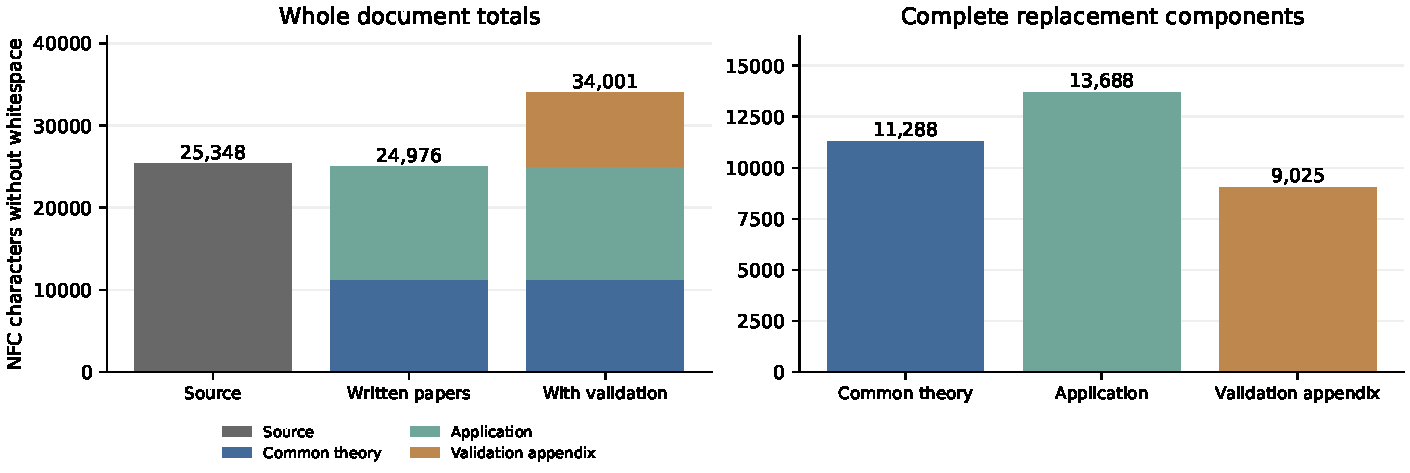
\includegraphics[width=\textwidth]{complete_costs.pdf}\end{center}
Both axes start at zero and every bar charges its complete documents.
The written difference in this ruler is only 372 characters;
the replacement including validation is longer than the source. A
single application supplies no evidence of a recurring sawtooth pattern.

\textbf{Sensitivity.}
For calibrated selected text in NFC:
\begin{center}\begin{tabular}{lrrr}\toprule
Unit & Written & Conditional & With appendix\\\midrule
Whitespace words & 1.008 & 1.831 & 0.896 \\
Alphanumeric units & 1.138 & 2.068 & 0.862 \\
Nonspace characters & 1.015 & 1.852 & 0.746 \\
Characters, spaces collapsed & 1.014 & 1.848 & 0.768 \\
UTF-8 bytes, spaces collapsed & 0.971 & 1.779 & 0.749 \\
\bottomrule\end{tabular}\end{center}
The UTF-8 written factor is below one: the small written saving is not
stable across these units. The full JSON and CSV retain all five units
under NFC and NFKC, each for untrimmed raw, selected raw and calibrated
selected text: thirty coordinates and 120 exact fractions. Printed
hyphens, code continuation marks and actual whitespace are preserved.

\textbf{Scope and retained costs.}
The current proofs correct the chamber degrees to $r-1$ and
$d(v)(r-1)$, the completed hexagon pair to $(D_{12},S_3)$, and the
symmetric-family minimum-degree statement to $n\geq3$. There is no
universal rank-two representation or blanket
$(S_n,A_n)=(\operatorname{Aut}(A_n),\operatorname{Inn}(A_n))$ claim.
The original Theorem A already answers Question 2.4; no new question
answer is claimed here.

The accepted independent input audit checked all 27 pages, 120 PDF
metric cells, sixty separate raw-file cells and 566 glyph classes in
26 actual font dictionaries. Its 134 visible-glyph repairs include
three byte-9 right braces; actual whitespace is otherwise preserved.
The four mapsto strokes remain separate from adjacent arrows. The ruler
uses pypdf 6.13.0 and FontTools 4.63.0. Source vector figures, edges,
colors and formula placement are not fully represented by extracted
text. Their cost, external proofs, historical software and operational
engineering remain unknown, not zero. These factors describe the
declared text representation, not total research effort or minimum
proof complexity. Independent numerical review is required before
publication.
\end{document}
